
\let\negmedspace\undefined
\let\negthickspace\undefined
\documentclass[journal,12pt,onecolumn]{IEEEtran}

\usepackage{cite}
\usepackage{amsmath,amssymb,amsfonts,amsthm}
\usepackage{algorithmic}
\usepackage{graphicx}
\graphicspath{{./figs/}}
\usepackage{textcomp}
\usepackage{xcolor}
\usepackage{txfonts}
\usepackage{listings}
\usepackage{enumitem}
\usepackage{mathtools}
\usepackage{gensymb}
\usepackage{comment}
\usepackage{caption}
\usepackage[breaklinks=true]{hyperref}
\usepackage{tkz-euclide}
\usepackage{listings}
\usepackage{gvv}
\usepackage[latin1]{inputenc}
\usepackage{xparse}
\usepackage{color}
\usepackage{array}
\usepackage{longtable}
\usepackage{calc}
\usepackage{multirow}
\usepackage{multicol}
\usepackage{hhline}
\usepackage{ifthen}
\usepackage{lscape}
\usepackage{tabularx}
\usepackage{array}
\usepackage{float}

\begin{document}

\title{10.7.69}
\author{EE25BTECH11020 - Darsh Pankaj Gajare}
{\let\newpage\relax\maketitle}

Question:\\

Let $x^2+y^2-4x-2y-11=0$ be a circle. A pair of tangents from the point $\brak{4,5}$ with a pair of radii form a quadrilateral with area\rule{1cm}{0.4pt}.


\solution
\begin{align}
\text{Conic: }\quad \vec{x}^\top V\vec{x}+2\vec{u}^\top\vec{x}+f=0
\end{align}

\begin{align}
V=\myvec{0 & 0\\[4pt]0 & 1},\quad \vec{u}=\myvec{-2\\[4pt]-1},\quad f=-11
\end{align}

Matrix equation of a line through P: 
\begin{align}
\vec{x}=\vec{P}+t\vec{m},\quad \vec{P}=\myvec{4\\5},\ \vec{m}=\myvec{1\\[4pt]k}
\end{align}
Substitute into the conic:
\begin{align}
	\brak{\vec{P}+t\vec{m}}^\top V\brak{\vec{P}+t\vec{m}}+2\vec{u}^\top\brak{\vec{P}+t\vec{m}}+f=0
\end{align}

\begin{align}
	\brak{k^2+1}t^2+\brak{8k+4}t+4=0
\end{align}

Tangency from P$\Rightarrow$ double root in $t$
\begin{align}
	\brak{8k+4}^2-4\cdot\brak{k^2+1}\cdot 4=0
\end{align}

\begin{align}
 k=0,-\frac{4}{3}
\end{align}

\begin{align}
\text{For each }k:\quad t=-\frac{8k+4}{2(k^2+1)}
\end{align}

\begin{align}
\text{Thus contact points }A=\vec{P}+t\vec{m}\text{ are }
A_1=\myvec{2\\5},\quad A_2=\myvec{\frac{26}{5}\\\frac{17}{5}}
\end{align}

\begin{align}
C=-\vec{u}=\myvec{2\\1}
\end{align}

\begin{align}
	area\brak{A_2CA_1P}=\frac{1}{2}\brak{\norm{\brak{\vec{A_1}-\vec{C}}\times\brak{\vec{P}-\vec{C}}}+\norm{\brak{\vec{A_2}-\vec{C}}\times\brak{\vec{P}-\vec{C}}}}=8
\end{align}

Plot using C libraries:
\begin{figure}[H]
	\centering
	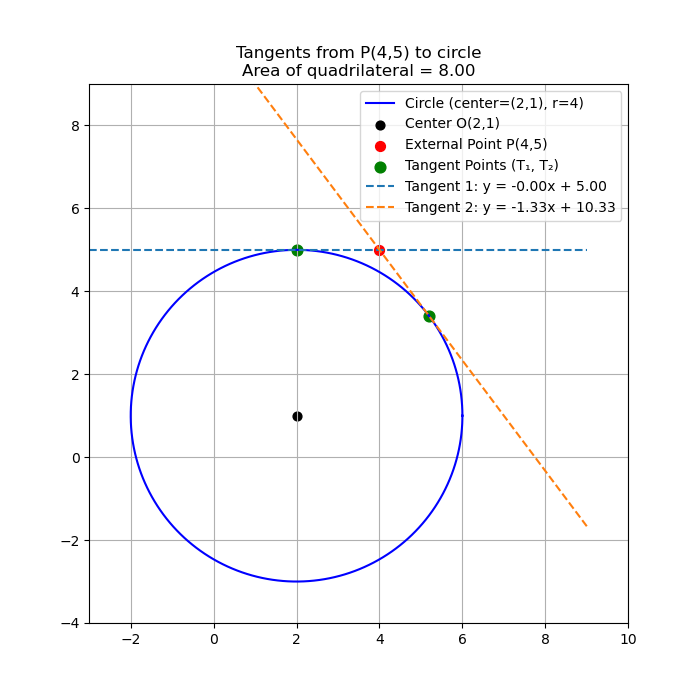
\includegraphics[scale=0.5]{img1}
	\caption*{}
	\label{img1}
\end{figure}
Plot using Python:
\begin{figure}[H]
	\centering
	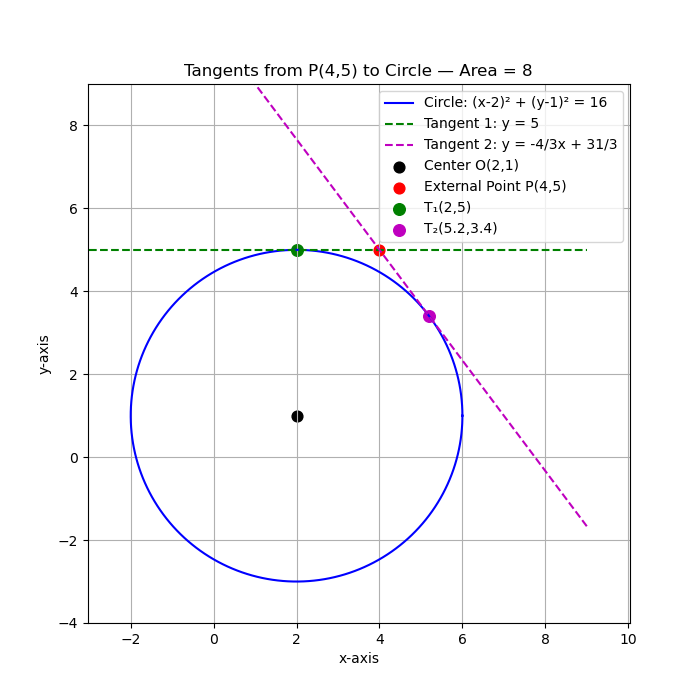
\includegraphics[scale=0.5]{img2}
	\caption*{}
	\label{img2}
\end{figure}

\end{document}
